%--------------------
% Packages
% -------------------
\documentclass[11pt,a4paper]{article}
\usepackage[utf8x]{inputenc}
\usepackage[T1]{fontenc}
\usepackage{mathpazo}
%\usepackage{gentium}
\usepackage{mathptmx} % Use Times Font


\usepackage[pdftex]{graphicx} % Required for including pictures
\usepackage[spanish]{babel} % Spanish translations
\usepackage[pdftex,linkcolor=black,pdfborder={0 0 0}]{hyperref} % Format links for pdf
\usepackage{calc} % To reset the counter in the document after title page
\usepackage{enumitem} % Includes lists

\frenchspacing % No double spacing between sentences
\linespread{1.2} % Set linespace
\usepackage[a4paper, lmargin=0.1666\paperwidth, rmargin=0.1666\paperwidth, tmargin=0.1111\paperheight, bmargin=0.1111\paperheight]{geometry} %margins
%\usepackage{parskip}

\usepackage[all]{nowidow} % Tries to remove widows
\usepackage[protrusion=true,expansion=true]{microtype} % Improves typography, load after fontpackage is selected

\graphicspath{{./figs/}}

\usepackage{float}
\usepackage{adjustbox}
\usepackage{xurl}
\usepackage{listings}

\usepackage{amsmath}
\usepackage{yhmath}

%-----------------------
% Set pdf information and add title, fill in the fields
%-----------------------
\hypersetup{ 	
pdfsubject = {},
pdftitle = {},
pdfauthor = {}
}

%-----------------------
% Begin document
%-----------------------
\begin{document} %All text i dokumentet hamnar mellan dessa taggar, allt ovanför är formatering av dokumentet

%----------------------------------------------------------------------------------------
%	TITLE PAGE
%----------------------------------------------------------------------------------------

\begin{titlepage} % Suppresses displaying the page number on the title page and the subsequent page counts as page 1
	\newcommand{\HRule}{\rule{\linewidth}{0.5mm}} % Defines a new command for horizontal lines, change thickness here
	
	\center % Centre everything on the page
	
	%------------------------------------------------
	%	Headings
	%------------------------------------------------
	
	\textsc{\LARGE Universidad de Castilla-La Mancha}\\[1.5cm] % Main heading such as the name of your university/college
	
	\textsc{\Large Minería de Datos}\\[0.5cm] % Major heading such as course name
	
	\textsc{\large Entregable Final}\\[0.5cm] % Minor heading such as course title
	
	%------------------------------------------------
	%	Title
	%------------------------------------------------
	
	\HRule\\[0.4cm]
	
	{\huge\bfseries Análisis de violencia con armas en EE. UU.}\\[0.4cm] % Title of your document
	
	\HRule\\[1.5cm]
	
	%------------------------------------------------
	%	Author(s)
	%------------------------------------------------
	
	\begin{minipage}{0.4\textwidth}
		\begin{flushleft}
            \textsc{Darío Andrés Fallavollita Figueroa}
		\end{flushleft}
        \begin{flushleft}
            \textsc{Fernando Potenciano Santiago}
        \end{flushleft}
		\begin{flushleft}
		  \textsc{Ignacio Rozas López}
		\end{flushleft}
	\end{minipage}
	~
	\begin{minipage}{0.4\textwidth}
        \begin{flushright}
            \textsc{Israel Mateos Aparicio Ruiz Santa Quiteria}
		\end{flushright}
        \begin{flushright}
            \textsc{Adrían Julián Ramos Romero}
        \end{flushright}
		\begin{flushright}
		  \textsc{Laurentiu Gheorghe Zlatar}
		\end{flushright}
	\end{minipage}
	
	% If you don't want a supervisor, uncomment the two lines below and comment the code above
	%{\large\textit{Author}}\\
	%John \textsc{Smith} % Your name
	
	%------------------------------------------------
	%	Date
	%------------------------------------------------
	
	\vfill\vfill\vfill % Position the date 3/4 down the remaining page
	
	{\large\today} % Date, change the \today to a set date if you want to be precise
	
	%------------------------------------------------
	%	Logo
	%------------------------------------------------
	
	%\vfill\vfill
	%\includegraphics[width=0.2\textwidth]{placeholder.jpg}\\[1cm] % Include a department/university logo - this will require the graphicx package
	 
	%----------------------------------------------------------------------------------------
	
	\vfill % Push the date up 1/4 of the remaining page
	
\end{titlepage}

%----------------------------------------------------------------------------------------

\tableofcontents

\newpage

\section{Porcentajes de participación}

El reparto de la participación entre integrantes ha sido equitativo, y se muestra en la tabla \ref{tab:participacion}.

\begin{table}[H]
    \centering
\adjustbox{max width=\textwidth}{
\begin{tabular}{|c|c|c|}
\hline
\textbf{Apellidos y nombre}                & \textbf{Correo}                      & \textbf{Participación} \\ \hline
Fallavollita Figueroa, Darío Andrés         & DarioAndres.Fallavollita@alu.uclm.es & 16,6\%                 \\ \hline
Mateos Aparicio Ruiz Santa Quiteria, Israel & Israel.Mateos@alu.uclm.es            & 16,6\%                 \\ \hline
Potenciano Santiago, Fernando               & Fernando.Potenciano@alu.uclm.es      & 16,6\%                 \\ \hline
Ramos Romero, Adrián Julián                 & AdrianJulian.Ramos@alu.uclm.es       & 16,6\%                 \\ \hline
Rozas López, Ignacio                        & Ignacio.Rozas@alu.uclm.es            & 16,6\%                 \\ \hline
Zlatar, Laurentiu Gheorghe                  & LaurentiuGheorghe.Zlatar@alu.uclm.es & 16,6\%                 \\ \hline
\end{tabular}
}
    \caption{Porcentaje de participación de los integrantes}
    \label{tab:participacion}
\end{table}

\section{Introducción}

El objetivo de este proyecto es el de analizar incidentes de violencia con armas en Estados Unidos, con el fin de encontrar patrones en ellos. Para ello, se tendrán en cuenta factores temporales, climáticos, demográficos y judiciales.

Siguiendo el proceso KDD, realizaremos los siguientes pasos:

\begin{enumerate}
    \item Obtendremos un conocimiento inicial del dominio y definiremos el problema. Esto lo haremos mediante la definición de una serie de hipótesis a probar.
    \item Determinaremos las fuentes de datos, y los obtendremos de estas.
    \item Preprocesaremos los datos para pasar de datos crudos a una o varias tarjetas de datos sobre las que aplicar algoritmos. Este paso puede descomponerse en:
    \begin{enumerate}
        \item Limpieza.
        \item Integración.
        \item Reducción.
        \item Transformación
    \end{enumerate}
    \item Aplicaremos algoritmos de minería de datos sobre nuestras tarjetas de datos para extraer patrones.
    \item Evaluaremos los resultados de los algoritmos mediante métricas y visualizaciones. Interpretaremos estos resultados y extraeremos el conocimiento deseado.
\end{enumerate}

\section{Dominio del problema y comprensión de objetivos}

El objetivo principal es el análisis de incidentes de violencia con armas en Estados Unidos. Se usarán datos con una granularidad de, como mínimo, estado y año. Para concretar más este objetivo general, hemos establecido cuatro hipótesis a probar:

\begin{itemize}
    \item Se producen más incidentes con armas los fines de semana.
    \item Se producen más incidentes con armas en los estados con climas más cálidos.
    \item Los incidentes con armas son más frecuentes en los estados con mayor pobreza.
    \item Cuantas más leyes sobre el uso de armas existen en un estado, menos incidentes con armas se producen en él.
\end{itemize}

Cada una de estas hipótesis corresponde a factores temporales, climáticos, demográficos y judiciales, respectivamente. Así, conseguimos dar una visión global del dominio del problema.

Inicialmente, la segunda hipótesis era ``Se producen más incidentes con armas en los meses de verano''. Sin embargo, por su parecido a la primera hipótesis (ambas tratan de buscar un patrón temporal en los datos) y su simplicidad, hemos decidido cambiarla por la que aquí se presenta. Esta nos permitirá un análisis de otro factor que no se tenía en cuenta, a la vez que usamos más fuentes de datos para enriquecer nuestro análisis.

Para ello hemos recopilado diferentes \textit{datasets}, siendo el principal datos sobre incidentes violentos con armas en EE.UU. Los demás serán secundarios, y contienen información sobre datos climáticos, de pobreza y de leyes para la regulación de las armas. Su función será enriquecer nuestro conjunto de datos principal y probar (o refutar) nuestras hipótesis iniciales, las cuales son:

\begin{itemize}
    \item Se producen más incidentes con armas los fines de semana.
    \item Se producen más incidentes con armas en los estados con climas más cálidos.
    \item Los incidentes con armas son más frecuentes en los estados con mayor pobreza.
    \item Cuantas más leyes sobre el uso de armas existen en un estado, menos incidentes con armas se producen en él.
\end{itemize}

Además, tras haber trabajado con los datos y ver algunos resultados, nos hemos dado cuenta de que el tema que vamos a afrontar es complejo, y que depende de muchos factores. Por ello, quizá obtenemos unos patrones al comparar cada dato con los incidentes independientemente de los demás, pero puedan cambiar si los analizamos todos en conjunto. Por ello, decidimos realizar un análisis extra en el que combinamos los datos climáticos, los de pobreza y los de leyes de regulación de armas. Los datos del número de incidentes en fines de semana y fuera de ellos no se han incluido en este análisis global, ya que presentan una granularidad distinta a la de todos los demás, además de parecernos el factor menos interesante.

\section{Recogida de datos}

Las fuentes principales de nuestros conjuntos de datos son las siguientes:

\begin{itemize}
    \item Incidentes violentos con armas en EE. UU: Obtenidos de \url{https://www.kaggle.com/datasets/jameslko/gun-violence-data} y cuya fuente original es \url{https://www.gunviolencearchive.org}.
    \item Datos de clima: Obtenidos del NOAA National Centers for Environmental Information (NCEI). Concretamente, los ficheros se encuentran en \url{https://www.ncei.noaa.gov/pub/data/cirs/climdiv/}.
    \item Datos de pobreza en EE.UU: Obtenidos mediante técnicas de \textit{web scraping} de \url{https://www.povertyusa.org/}
    \item Leyes para armas de fuego en EE. UU: Obtenidos directamente de \url{https://mail.statefirearmlaws.org/}.
\end{itemize}

Además, en pasos posteriores nos hemos dado cuenta de que sería una buena idea escalar el número de incidentes en un estado por sus habitantes, ya que estos están relacionados y provocan grandes diferencias en el número de incidentes entre estados. Por ello, y ya que KDD es un proceso iterativo, hemos vuelto a este paso para integrar un conjunto de datos más.

Este conjunto de datos se compone de datos de poblaciones para los distintos estados de EE. UU. Es obtenido directamente de la Oficina del Censo de los Estados Unidos (\textit{U.S. Census Bureau}), concretamente de \url{https://www2.census.gov/programs-surveys/popest/datasets/2010-2019/national/totals/nst-est2019-alldata.csv}.

\subsection{Descripción breve de los datos originales}

A continuación se presentan los diccionarios de datos para cada uno de ellos a modo de descripción. Si no es posible dar estos diccionarios de datos por presentar un formato atípico, se hace una breve descripción de los ficheros que contienen los datos y su formato.

\subsubsection*{Incidentes violentos con armas en EE. UU.}

El conjunto de datos principal trata sobre incidentes violentos con armas en EE. UU., obtenido de \url{https://www.kaggle.com/datasets/jameslko/gun-violence-data}. Se muestra en la tabla \ref{tab:dict_datos_incidentes}.

\begin{table}[H]
    \centering
\adjustbox{max width=\textwidth}{
\begin{tabular}{|c|c|c|}
\hline
\textbf{Columna}               & \textbf{Tipo de dato} & \textbf{Descripción}                                                                                                             \\ \hline
incident\_id                   & int                   & Identificador del incidente                                                                                                      \\ \hline
date                           & date                  & Fecha en la que se produjo el crimen                                                                                             \\ \hline
state                          & String                & Estado en el que se produjo el crimen                                                                                            \\ \hline
city\_or\_county               & String                & Ciudad/condado del crimen                                                                                                        \\ \hline
address                        & String                & Dirección del lugar del crimen                                                                                                   \\ \hline
n\_killed                      & int                   & Número de personas fallecidas                                                                                                    \\ \hline
n\_injured                     & int                   & Número de personas heridas                                                                                                       \\ \hline
incident\_url                  & url                   & URL acerca del incidente                                                                                                         \\ \hline
source\_url                    & String                & Referencia a la fuente del informe                                                                                               \\ \hline
incident\_url\_fields\_missing & boolean               & \begin{tabular}[c]{@{}c@{}}Validación del URL: verdadero si incident\_url\\ está presente, falso en caso contrario\end{tabular}  \\ \hline
congressional\_district        & int                   & Identificador del distrito electoral                                                                                             \\ \hline
gun\_stolen                    & String                & Estado de las armas involucradas en el crimen.                                                                                   \\ \hline
gun\_type                      & String                & Tipificación de las armas utilizadas en el crimen                                                                                \\ \hline
incident\_characteristics      & String                & Características del incidente                                                                                                    \\ \hline
latitude                       & float                 & Distancia de latitud                                                                                                             \\ \hline
location\_description          & String                & Localización concreta del incidente                                                                                              \\ \hline
longitude                      & float                 & Distancia de longitud                                                                                                            \\ \hline
n\_guns\_involved              & int                   & Número de armas involucradas en el incidente                                                                                     \\ \hline
notes                          & int                   & Información adicional del crimen                                                                                                 \\ \hline
participant\_age               & String                & Edad exacta de los participantes en el momento del crimen                                                                        \\ \hline
participant\_age\_group        & String                & Grupo de edad de los participantes en el momento del crimen                                                                      \\ \hline
participant\_gender            & String                & Género de los participantes                                                                                                      \\ \hline
participant\_name              & String                & Nombre de los participantes involucrados en el crimen                                                                            \\ \hline
participant\_relationship      & String                & Relación del participante con otros participantes                                                                                \\ \hline
participant\_status            & String                & Grado de daño hecho al participante                                                                                              \\ \hline
participant\_type              & String                & Papel del involucrado en el crimen                                                                                               \\ \hline
sources                        & url                   & Fuente de los participantes                                                                                                      \\ \hline
state\_house\_district         & int                   & \begin{tabular}[c]{@{}c@{}}Distrito electoral de la cámara de representantes\\ para la elección de un representante\end{tabular} \\ \hline
state\_senate\_district        & int                   & \begin{tabular}[c]{@{}c@{}}Distrito electoral para elección de un senador\\ estatal en una legislatura\end{tabular}              \\ \hline
\end{tabular}
}
    \caption{Diccionario de datos del conjunto de datos de incidentes violentos con armas en EE. UU.}
    \label{tab:dict_datos_incidentes}
\end{table}

\subsubsection*{Datos de clima en EE. UU.}

El conjunto de datos que trata acerca de datos climáticos en EE. UU. se ha obtenido de \url{https://www.ncei.noaa.gov/pub/data/cirs/climdiv/}. A diferencia de los demás conjuntos de datos, este no presenta un formato de tabla, sino que se provee en dos ficheros de texto (uno para datos de temperatura y otro para datos de precipitaciones) con un formato específico. Este formato consiste en que cada línea se compone de una primera palabra con un código que representa el estado, la magnitud medida, el año..., y las siguientes doce palabras corresponden a esa medida para cada mes (de izquierda a derecha: enero, febrero...). Las palabras están separadas por varios espacios en blanco.

Además, el código utilizado para identificar estados no es un código estándar como el código FIPS, sino que es un código propio del NCEI. Por tanto, se ha descargado también otro fichero de la misma fuente donde se describen todos los datos. De este se extraerá posteriormente la sección de códigos de estado.

\subsubsection*{Datos de pobreza en EE. UU.}

El conjunto de datos que trata acerca de datos de pobreza en EE. UU. se ha obtenido de \url{https://www.povertyusa.org/data}. Se muestra en la tabla \ref{tab:dict_datos_pobreza}.

\begin{table}[H]
    \centering
\adjustbox{max width=\textwidth}{
\begin{tabular}{|c|c|c|}
\hline
\textbf{Columna}               & \textbf{Tipo de dato} & \textbf{Descripción}                                                                                                                                                                                                                                                                                                                                                                                                                                  \\ \hline
year                           & int                   & El año al que corresponde la información en el registro                                                                                                                                                                                                                                                                                                                                                                                               \\ \hline
state                          & String                & El estado de Estados Unidos al que se refiere el registro                                                                                                                                                                                                                                                                                                                                                                                             \\ \hline
population                     & int                   & La población total en el estado y año especificados                                                                                                                                                                                                                                                                                                                                                                                                   \\ \hline
in\_poverty                    & int                   & \begin{tabular}[c]{@{}c@{}}El número de personas que se encuentran en situación de pobreza\\      (ganan menos que el umbral de pobreza oficial del gobierno, que\\      para una familia de cuatro miembros es de unos 25,700 dólares)\end{tabular}                                                                                                                                                                                                  \\ \hline
poverty\_rate                  & float                 & \begin{tabular}[c]{@{}c@{}}La tasa de pobreza, expresada como un porcentaje, que representa la\\      proporción de la población que se encuentra en situación de pobreza\end{tabular}                                                                                                                                                                                                                                                                \\ \hline
median\_household\_income      & float                 & \begin{tabular}[c]{@{}c@{}}La mediana de los ingresos de los hogares. Incluye los ingresos del\\      cabeza de familia y de todas las demás personas de 15 años o más\\      del hogar, estén o no emparentadas con el cabeza de familia\end{tabular}                                                                                                                                                                                                \\ \hline
deep\_poverty\_rate            & float                 & \begin{tabular}[c]{@{}c@{}}Porcentaje de personas que viven en un hogar con unos ingresos\\      totales en efectivo inferiores al 50\% del umbral de pobreza\\      establecido por la Oficina del Censo de Estados Unidos\end{tabular}                                                                                                                                                                                                              \\ \hline
median\_rent                   & float                 & \begin{tabular}[c]{@{}c@{}}La mediana de los costos del alquiler y los servicios\\      de una vivienda de dos dormitorios\end{tabular}                                                                                                                                                                                                                                                                                                               \\ \hline
unemployment\_rate             & float                 & \begin{tabular}[c]{@{}c@{}}Porcentaje de trabajadores desempleados que han buscado trabajo\\      activamente y están actualmente disponibles para trabajar\end{tabular}                                                                                                                                                                                                                                                                              \\ \hline
without\_health\_insurance     & float                 & \begin{tabular}[c]{@{}c@{}}Porcentaje de personas menores de 65 años y por debajo\\      del 138\% del umbral de pobreza que no tenían seguro\\      médico en ningún momento del año\end{tabular}                                                                                                                                                                                                                                                    \\ \hline
supplemental\_poverty\_measure & float                 & \begin{tabular}[c]{@{}c@{}}La Medida de Pobreza Suplementaria (SPM) tiene en cuenta a\\      las personas que caerían en la pobreza sin ciertas prestaciones\\      no monetarias que les ayudan a superar el umbral de pobreza.\\      Estas prestaciones incluyen la ayuda alimentaria y los subsidios\\      de alquiler, así como las ayudas basadas en los impuestos,\\      como el crédito fiscal por ingresos del trabajo (EITC)\end{tabular} \\ \hline
\end{tabular}
}
    \caption{Diccionario de datos del conjunto de datos de pobreza en EE. UU.}
    \label{tab:dict_datos_pobreza}
\end{table}

\subsubsection*{Leyes para armas de fuego en EE. UU.}

Los conjuntos de datos que tratan acerca de datos de leyes sobre armas de fuego en EE. UU. se han obtenido de \url{https://mail.statefirearmlaws.org/resources}.

En realidad, se trata de un único conjunto de datos, mostrado en la tabla \ref{tab:dict_datos_leyes_ds}, mientras que el mostrado en la tabla \ref{tab:dict_datos_leyes_cb} se trata de un \textit{codebook} acerca del primero. Sin embargo, este último contiene una categorización de las leyes, que nos puede ser útil para analizar la importancia de cada una de estas categorías por separado. Por tanto, se incluyen ambos. 

\begin{table}[H]
    \centering
\begin{tabular}{|c|c|c|}
\hline
\textbf{Columna}           & \textbf{Tipo de dato} & \textbf{Descripción}                                                                                       \\ \hline
state                      & String                & \begin{tabular}[c]{@{}c@{}}Estado de EE. UU. al que corresponde\\ la información del registro\end{tabular} \\ \hline
year                       & int                   & \begin{tabular}[c]{@{}c@{}}Año al que corresponde la\\ información del registro\end{tabular}               \\ \hline
felony, invcommitment, ... & boolean               & Ley concreta que puede o no estar vigente                                                                  \\ \hline
lawtotal                   & int                   & Cantidad total de leyes vigentes                                                                           \\ \hline
\end{tabular}
    \caption{Diccionario de datos del conjunto de datos de leyes para armas de fuego en EE. UU.}
    \label{tab:dict_datos_leyes_ds}
\end{table}

\begin{table}[H]
    \centering
\adjustbox{max width=\textwidth}{
\begin{tabular}{|c|c|c|}
\hline
\textbf{Columna}                  & \textbf{Tipo de dato} & \textbf{Descripción}                                                                                                                                           \\ \hline
Category Code                     & int                   & Identificador de categoría de leyes                                                                                                                            \\ \hline
Category                          & String                & Categoría de la ley                                                                                                                                            \\ \hline
Sub-Category                      & String                & Subcategoría de la ley                                                                                                                                         \\ \hline
Variable Name                     & String                & \begin{tabular}[c]{@{}c@{}}Nombre de la ley en el anterior\\ conjunto de datos. Corresponden a las\\ definidas anteriormente: felony, danger, ...\end{tabular} \\ \hline
Brief Description of Provision    & String                & Descripción breve de la ley                                                                                                                                    \\ \hline
Detailed Description of Provision & String                & Descripción detallada de la ley                                                                                                                                \\ \hline
Coding Notes                      & String                & \begin{tabular}[c]{@{}c@{}}Notas adicionales para asignar un valor\\ (vigente o no vigente) a cada ley\end{tabular}                                            \\ \hline
Coding Instructions               & String                & \begin{tabular}[c]{@{}c@{}}Instrucciones de qué valor asignar\\ (vigente o no vigente) a cada ley\end{tabular}                                                 \\ \hline
Notes                             & String                & Notas adicionales                                                                                                                                              \\ \hline
Data Source and Attribution       & String                & Fuente de todos los datos y autores                                                                                                                            \\ \hline
\end{tabular}
}
    \caption{Diccionario de datos del \textit{codebook} del conjunto de datos de leyes para armas de fuego en EE. UU.}
    \label{tab:dict_datos_leyes_cb}
\end{table}

\subsubsection*{Datos de poblaciones en EE. UU.}

El conjunto de datos que tratan acerca de poblaciones se ha obtenido de \url{https://www2.census.gov/programs-surveys/popest/datasets/2010-2019/national/totals/nst-est2019-alldata.csv} y se muestra en la tabla \ref{tab:dict_datos_pobl}.

Las columnas que contiene un rango de tiempo, i.e. POPESTIMATE2010-2019, NPOPC\-HG2010-2019..., son en realidad una columna por año, i.e. POPESTIMATE2010, POPESTIMATE2011, POPESTIMATE2012... Para hacer la descripción más clara y concisa se han agrupado, ya que tienen el mismo significado.

\begin{table}[H]
    \centering
\adjustbox{max width=\textwidth}{
\begin{tabular}{|c|c|c|}
\hline
\textbf{Columna}           & \textbf{Tipo de dato} & \textbf{Descripción}                                                                                               \\ \hline
SUMLEV                     & int                   & Nivel de resumen geográfico                                                                                        \\ \hline
REGION                     & int                   & Código de Región del Censo                                                                                         \\ \hline
DIVISION                   & int                   & Código de División del Censo                                                                                       \\ \hline
STATE                      & int                   & Código FIPS del Estado                                                                                             \\ \hline
NAME                       & String                & Nombre del Estado                                                                                                  \\ \hline
CENSUS2010POP              & int                   & Población total residente del Censo 2010                                                                           \\ \hline
ESTIMATESBASE2010          & int                   & Población total estimada base al 4/1/2010                                                                          \\ \hline
POPESTIMATE2010-2019       & int                   & \begin{tabular}[c]{@{}c@{}}Estimación de población total\\ residente al 7/1/2010-7/1/2019\end{tabular}             \\ \hline
NPOPCHG\_2010-2019         & int                   & \begin{tabular}[c]{@{}c@{}}Cambio numérico en la población\\ total residente 4/1/2010-7/1/2019\end{tabular}        \\ \hline
BIRTHS2010-2019            & int                   & \begin{tabular}[c]{@{}c@{}}Nacimientos en el periodo\\ 4/1/2010 al 6/30/2019\end{tabular}                          \\ \hline
DEATHS2010-2019            & int                   & \begin{tabular}[c]{@{}c@{}}Defunciones en el periodo\\ 4/1/2010 al 6/30/2019\end{tabular}                          \\ \hline
NATURALINC2010-2019        & int                   & \begin{tabular}[c]{@{}c@{}}Incremento natural en el periodo\\ 4/1/2010 al 6/30/2019\end{tabular}                   \\ \hline
INTERNATIONALMIG2010-2019  & int                   & \begin{tabular}[c]{@{}c@{}}Migración internacional neta en\\ el periodo 4/1/2010 al 6/30/2019\end{tabular}         \\ \hline
DOMESTICMIG2010-2019       & int                   & \begin{tabular}[c]{@{}c@{}}Migración doméstica neta en\\ el periodo 4/1/2010 al 6/30/2019\end{tabular}             \\ \hline
NETMIG2010-2019            & int                   & \begin{tabular}[c]{@{}c@{}}Migración neta en el periodo\\ 4/1/2010 al 6/30/2019\end{tabular}                       \\ \hline
RESIDUAL2010-2019          & int                   & \begin{tabular}[c]{@{}c@{}}Residual para el periodo\\ 4/1/2010 al 6/30/2019\end{tabular}                           \\ \hline
RBIRTH2011-2019            & float                 & \begin{tabular}[c]{@{}c@{}}Tasa de natalidad en el periodo\\ 7/1/2010 al 6/30/2019\end{tabular}                    \\ \hline
RDEATH2011-2019            & float                 & \begin{tabular}[c]{@{}c@{}}Tasa de mortalidad en el periodo\\ 7/1/2010 al 6/30/2019\end{tabular}                   \\ \hline
RNATURALINC2011-2019       & float                 & \begin{tabular}[c]{@{}c@{}}Tasa de incremento natural en el\\ periodo 7/1/2010 al 6/30/2019\end{tabular}           \\ \hline
RINTERNATIONALMIG2011-2019 & float                 & \begin{tabular}[c]{@{}c@{}}Tasa de migración internacional neta\\ en el periodo 7/1/2010 al 6/30/2019\end{tabular} \\ \hline
RDOMESTICMIG2011-2019      & float                 & \begin{tabular}[c]{@{}c@{}}Tasa de migración doméstica neta\\ en el periodo 7/1/2010 al 6/30/2019\end{tabular}     \\ \hline
RNETMIG2011-2019           & float                 & \begin{tabular}[c]{@{}c@{}}Tasa de migración neta en el\\ periodo 7/1/2010 al 6/30/2019\end{tabular}               \\ \hline
\end{tabular}
}
    \caption{Diccionario de datos del conjunto de datos de poblaciones de EE. UU.}
    \label{tab:dict_datos_pobl}
\end{table}

\section{Preproceso y transformación}

\subsection{Incidentes con armas}

Nuestro conjunto de datos de incidentes con armas viene dado en un único fichero, en el que cada registro corresponde a un incidente en un estado y fecha concretos. Ya que las columnas que seleccionaremos no contienen nulos, y \textit{a priori} estos están relativamente limpios, hemos decidido limpiar el conjunto de datos al completo, aunque después solo seleccionaremos algunas columnas. Esto es con el fin de mostrar que somos capaces de limpiar un conjunto de datos de un tamaño considerable.

En el primer paso de nuestra limpieza, nos encontramos con nulos en varias columnas. La estrategia general a seguir ha sido la de imputar estos valores con la media de la variable en caso de ser numérica o la moda en caso de ser categórica. Sin embargo, nos hemos encontrado con algunos casos particulares en los que hemos seguido otra estrategia:

\begin{itemize}
    \item En las variables con más de un 50\% de nulos se ha imputado un valor \textit{Unknown}, por no ser el estadístico una medida representativa de todo el conjunto de datos.
    
    \item Varias columnas presentan un formato de texto propio. Por ejemplo, la variable \textit{gun\_type} presenta una única cadena de texto, en la que se especifica el tipo de cada arma involucrada (presentando así una dependencia con la variable \textit{n\_guns involved}.

    En estas variables se han extraído los valores individuales del formato que usa, se ha aplicado la estrategia de media o moda según el tipo de variable, y se han imputado estos valores siguiendo de nuevo el formato concreto.

    Esto ocurre con las variables relacionadas con las armas involucradas y con datos de los participantes del incidente.

    \item En variables en las que no tiene sentido utilizar la media o la moda, y que presentan un gran porcentaje de valores únicos (por ejemplo, \textit{notes} o \textit{address}, se ha imputado el valor \textit{Unknown}.

    \item Para las variables de latitud y longitud, por contener información espacial muy concreta, se ha usado la media para el estado en concreto en lugar de la media para toda la variable.

    \item Para las variables de distrito, se ha usado la moda para el estado en concreto, por tener este valor un significado distinto dependiendo del distrito.
\end{itemize}

Respecto al tratamiento de \textit{outliers}, se han controlado los de las variables numéricas exceptuando el identificador del incidente por ser una variable única, y de la latitud y longitud por estar en un contexto geográfica muy amplio (la totalidad de los Estados Unidos).

Tras analizarlos, se han encontrado valores extremos como edades de 300 años (claramente erróneos) e incidentes con más de 300 armas involucradas. Gracias a este análisis, hemos observado que el conjunto de datos incluye como incidentes ciertas acciones del gobierno tales como confiscaciones masivas y operaciones de \textit{gun buyback}. Este tipo de incidentes no tiene relevancia para nuestro objetivo y, de hecho, introduciría ruido en el mismo. Por tanto, hemos decidido eliminar los valores que distan más de 3 desviaciones estándar de la media de la variable.

Respecto a la integración, hemos separado las fechas en las variables \textit{year}, \textit{month} y \textit{day} para poder trabajar con otros conjuntos de datos que presentan una granularidad de año o mes. También hemos convertido las variables que presentaban el formato propio anteriormente mencionado en listas con los valores individuales, que es lo que realmente nos interesa.

Finalmente, hemos seleccionado las variables de fecha y estado, ya que para nuestro análisis lo único que nos interesa es el número de incidentes. También hemos descartado los datos de 2018, pues solo presentan incidentes hasta marzo. Además, para las hipótesis en las que haya que usar también datos de pobreza descartaremos los datos previos al 2015, ya que estos datos comienzan en ese año. A su vez, cuando se usen en conjunto con los datos de leyes, se descartaran los datos del estado "District of Columbia", ya que no tenemos datos de leyes para ese estado. Cuando se usen en conjunto con los datos climáticos, se descartarán los datos de los estados "District of Columbia" y "Hawaii" por la misma razón.

\subsection{Datos de clima}

Respecto a los datos de clima, necesitábamos pasar primero a un formato con el que pudiésemos trabajar antes de limpiarlos. El formato inicial contiene un código identificador propio de cada línea junto con los valores para cada mes, que puede observarse en el listado \ref{lst:format_clima}.

\begin{lstlisting}[language=,caption={Muestra del formato de datos de clima}]
    0010021895  43.10  37.40  54.50  63.40  69.50  ...
    0010021896  43.50  47.70  52.50  68.00  75.90  ...
    0010021897  41.80  51.10  60.20  62.40  69.00  ...
\end{lstlisting}
\label{lst:format_clima}

Mediante un \textit{parseo} del fichero, logramos poner los datos en un formato de tabla adecuado, combinando tanto temperatura como precipitaciones, como puede verse en la tabla \ref{tab:format_clima_processed}.

\begin{table}[H]
    \centering
\begin{tabular}{|ccccc|}
\hline
\multicolumn{1}{|c|}{\textbf{state}} & \multicolumn{1}{c|}{\textbf{year}} & \multicolumn{1}{c|}{\textbf{month}} & \multicolumn{1}{c|}{\textbf{average\_temperature}} & \textbf{average\_precipitation} \\ \hline
\multicolumn{1}{|c|}{Alabama}        & \multicolumn{1}{c|}{1895}          & \multicolumn{1}{c|}{1}              & \multicolumn{1}{c|}{43.10}                         & 7.52                            \\ \hline
\multicolumn{1}{|c|}{Alabama}        & \multicolumn{1}{c|}{1895}          & \multicolumn{1}{c|}{2}              & \multicolumn{1}{c|}{43.50}                         & 2.68                            \\ \hline
\multicolumn{1}{|c|}{Alabama}        & \multicolumn{1}{c|}{1895}          & \multicolumn{1}{c|}{3}              & \multicolumn{1}{c|}{41.80}                         & 7.64                            \\ \hline
\multicolumn{5}{|c|}{...}                                                                                                                                                                              \\ \hline
\end{tabular}
    \caption{Datos de clima formateados adecuadamente}
    \label{tab:format_clima_processed}
\end{table}

Estas operaciones previas corresponderían a la parte de integración, pero se ha realizado antes por ser necesario para trabajar con los datos.

Una vez formateados los datos correctamente, los datos faltantes en temperatura y precipitaciones se han rellenado con la media de la variable para el estado correspondiente. Los valores extremos se encuentran en proporciones menores al 1\%, y pueden ser interesantes para detectar patrones en estados muy fríos, con poca lluvia..., por lo que no se han eliminado ni sustituido.

Además, los datos de temperatura están en grados Fahrenheit y los de precipitaciones en centésimas de pulgada. Para facilitar su entendimiento, los hemos convertido a grados Celsius y a milímetros (o, lo que es lo mismo, litros por metro cuadrado), respectivamente.

Finalmente, se han descartado los datos anteriores a 2014 y posteriores a 2018, ya que no tenemos datos de incidentes para esos años.

\subsection{Datos de pobreza}

Respecto a la limpieza del conjunto de datos de pobreza, nos hemos encontrado con casos puntuales de nulos, que hemos reemplazado por la media (por ser numéricas) de la variable en el estado en concreto. Ya que son datos demográficos, dependen de la situación socioeconómica concreta de cada estado, por lo que no hemos usado la media de la variable completa (que correspondería a los Estados Unidos).

En lo que respecta a los valores extremos, la mayoría de nuestras variables consisten de porcentajes, por lo que están escaladas del 0 al 1. Por esta razón, ninguna de estas variables presenta valores extremos. Por el contrario, otras variables como la población o el número de habitantes viviendo en estado de pobreza si que presentan algunos. Sin embargo, para nuestro análisis usaremos porcentajes respecto a la población (por las diferencias en esta de un estado a otro, e.g. de Alaska a California), por lo que hemos decidido no eliminar los \textit{outliers} de esas variables del conjunto de datos.

Los datos de este conjunto presentan un formato adecuado para su integración con los demás, por lo que se ha pasado a la selección directamente.

Aunque a primera vista pensabamos que todos los indicadores de pobreza presentes en el conjunto de datos eran interesantes para nuestro análisis, tras analizar la correlación entre las distintas variables nos hemos dado cuenta de que existe una fuerte correlación entre todos los indicadores. Por tanto, hemos decidido quedarnos con sólo uno de ellos. Este ha sido el porcentaje de la población viviendo en estado de pobreza, por ser el más general.

\subsection{Leyes de regulación de armas}

Respecto al conjunto de datos acerca de leyes reguladoras de las armas, nos encontramos ante unos datos algo distintos. Cada registro del conjunto de datos se refiere a un estado y año concreto, y presenta una variable por cada ley, con un valor de 1 si está activa o de 0 en caso contrario, además de una variable con la cantidad de leyes activas. Además, hacemos uso de un \textit{codebook} (diccionario de datos) en el que cada ley está categorizada.

Este \textit{codebook} presenta valores nulos en variables referentes a anotaciones sobre la ley que no nos son de interés. En estas, se ha imputado un valor \textit{Unknown}. Respecto a los valores extremos, el \textit{codebook} solo presenta variables categóricas, mientras que el conjunto de datos en sí solo presenta variables categóricas o booleanas, a excepción de la cantidad total de leyes en cada estado y año. Por tanto, no se ha realizado ninguna operación respecto a \textit{outliers}.

Para facilitar el manejo del conjunto de datos en su posterior integración con los demás, se han cambiado los nombres de las columnas al mismo formato que las demás, i.e. en minúscula y usando guiones bajos como separados.

Se han seleccionado sólo el código de la categoría y los nombres de las variables de cada ley para el \textit{codebook}, y todas las variables para el conjunto de datos en sí, ya que posteriormente agruparemos las leyes por su categoría. Además, se han descartado los datos previos a 2014 para coincidir con los datos de incidentes.

\subsection{Datos de población}

Respecto a la limpieza del conjunto de datos de población, que no se usarán directamente sino para escalar los incidentes por los habitantes de cada estado, no nos hemos encontrado con valores nulos. Los \textit{outliers} tampoco han sido ni eliminados ni sustituidos, ya que necesitamos estos datos de poblaciones para escalar.

Para los distintos indicadores de población, el conjunto presenta una variable para cada indicador y año. Para su integración con los demás conjuntos de datos, hemos creado una variable para el año y modificado las demás columnas, de manera que obtengamos una única columna para cada indicador.

Una vez modificada la estructura del conjunto de datos, hemos visto que existen valores nulos para todos los datos de 2010 en algunos indicadores. Previamente, al tener una columna por indicador y por año, no existía la columna para 2010 de estos indicadores. Por esa razón, no detectamos estos nulos. Ahora, por tanto, volvemos a la fase de limpieza, y tratamos estos nulos reemplazándolos por la media de la variable para el estado en concreto.

Por último, hemos descartado datos de poblaciones de Puerto Rico, y datos que agrupan las poblaciones para ciertas regiones, así como los que las agrupan a nivel nacional. También hemos descartado datos fuera del rango de 2014 a 2017. Así, haremos que coincidan con los datos de incidentes.

\subsection{Transformación}

Una vez hemos limpiado los conjuntos de datos, hemos dado un formato común y que nos es útil, y hemos seleccionado los datos que necesitamos, hemos pasado a la transformación de los datos para la generación de las tarjetas de datos.

Ya que nuestras hipótesis necesitan de distintos conjuntos y distintas granularidades a nivel temporal, hemos decidido crear una tarjeta de datos para cada hipótesis.

Para la tarjeta de datos de la primera hipótesis, que trata del análisis del número de incidentes en fines de semana, hemos creado una nueva variable en función de la información que tenemos: indica si el incidente en concreto se produce o no en fin de semana. Mediante esta variable, después hemos agrupado el conjunto por estado, año y si es fin de semana. Ya que hay más días fuera del fin de semana que en ellos hemos escalado el número de incidentes dividiéndolo por el número de días en el que se dan. Además, hemos dividido este número de incidentes por cada 100.000 habitantes, con el fin de que nuestros datos sean más independientes respecto al estado.

Para la tarjeta de datos de la segunda hipótesis, que trata del análisis de la relación entre incidentes y datos climáticos, hemos agregado los incidentes a nivel de estado, año y mes, ya que los datos climáticos tienen una granularidad mensual. Además, hemos dividido este número de incidentes por cada 100.000 habitantes, con el fin de escalar nuestros datos.

Para la tarjeta de datos de la tercera hipótesis, que trata del análisis de la relación entre incidentes y datos de pobreza, hemos agregado los incidentes a nivel de estado y año. También hemos dividido este número de incidentes por cada 100.000 habitantes de la misma manera que en la segunda tarjeta de datos.

Para la tarjeta de datos de la cuarta y última hipótesis, que trata del análisis de la relación entre incidentes y leyes reguladoras de armas, hemos agregado de nuevo los incidentes por estado y año. Hemos creado también una nueva variable por cada categoría de ley, y hemos asignado a cada una de ellas el número de leyes activas de esa categoría. También hemos añadido la variable con el número total de leyes activas, y hemos escalado el número de incidentes de la misma manera que en la segunda y tercera tarjeta de datos.

Por último, hemos generado otra tarjeta de datos para el análisis extra en el que combinamos todos los datos excepto los incidentes en fin de semana o fuera de estos, por tener una granularidad y un escalado (ambos por día) diferentes. Para esta última tarjeta de datos, hemos agregado todos los datos por estado y año (algunos, como los climáticos, tenían una granularidad mensual). Hemos usado las nuevas variables generadas en las tarjetas de datos para las hipótesis 2, 3 y 4, y hemos vuelto a escalar los incidentes por cada 100.000 habitantes.

Estas tarjetas de datos se muestran con más claridad en la siguiente sección del documento.

\subsection{Características de la tarjeta de datos}

Como se ha explicado en la sección anterior, hemos decidido crear una tarjeta de datos para las dos primeras hipótesis y otra por cada una de las restantes.

A continuación, mostramos los diccionarios de datos para cada una de las tarjetas de datos.

\subsubsection*{Hipótesis 1: fines de semana}

Para la primera hipótesis, la tarjeta de datos presenta las variables mostradas en la tabla \ref{tab:datacard_h1}.

\begin{table}[H]
    \centering
\begin{tabular}{|c|c|c|}
\hline
\textbf{Columna}       & \textbf{Tipo de dato} & \textbf{Descripción}                                                                                                            \\ \hline
state                  & String                & Estado al que se refiere el registro                                                                                            \\ \hline
year                   & int                   & Año al que se refiere el registro                                                                                               \\ \hline
is\_weekend            & int                   & \begin{tabular}[c]{@{}c@{}}1 si se refiere a incidentes producidos\\ en fin de semana, 0 en caso contrario\end{tabular}         \\ \hline
n\_incidents\_per\_day & float                 & \begin{tabular}[c]{@{}c@{}}Número de incidentes con armas al día\\ por cada 100.000 habitantes, 0 en caso contrario\end{tabular}                                                                                           \\ \hline
\end{tabular}
    \caption{Diccionario de la tarjeta de datos para la hipótesis 1}
    \label{tab:datacard_h1}
\end{table}

\subsubsection*{Hipótesis 2: datos climáticos}

Para la segunda hipótesis, la tarjeta de datos presenta las variables mostradas en la tabla \ref{tab:datacard_h2}.

\begin{table}[H]
    \centering
\begin{tabular}{|c|c|c|}
\hline
\textbf{Columna}       & \textbf{Tipo de dato} & \textbf{Descripción}                   \\ \hline
state                  & String                & Estado al que se refiere el registro   \\ \hline
year                   & int                   & Año al que se refiere el registro      \\ \hline
month                  & int                   & Mes al que se refiere el registro      \\ \hline
n\_incidents           & float                 & Número de incidentes por 100.000 habitantes   \\ \hline
average\_temperature   & float                 & Temperatura media mensual en Celsius   \\ \hline
average\_precipitation & float                 & Precipitaciones medias mensuales en mm \\ \hline
\end{tabular}
    \caption{Diccionario de la tarjeta de datos para la hipótesis 2}
    \label{tab:datacard_h2}
\end{table}

\subsubsection*{Hipótesis 3: datos de pobreza}

Para la tercera hipótesis, la tarjeta de datos presenta las variables mostradas en la tabla \ref{tab:datacard_h3}.

\begin{table}[H]
    \centering
\begin{tabular}{|c|c|c|}
\hline
\textbf{Columna} & \textbf{Tipo de dato} & \textbf{Descripción}                                                                                                                                                                                         \\ \hline
state            & String                & Estado al que se refiere el registro                                                                                                                                                                         \\ \hline
year             & int                   & Año al que se refiere el registro                                                                                                                                                                            \\ \hline
n\_incidents     & float                 & Número de incidentes por 100.000 habitantes                                                                                                                                                                  \\ \hline
poverty\_rate    & float                 & \begin{tabular}[c]{@{}c@{}}La tasa de pobreza, que representa el porcentaje de\\ la población viviendo por debajo del umbral de pobreza\\ (para una familia de 4 miembros, unos 27.500 dólares)\end{tabular} \\ \hline
\end{tabular}
    \caption{Diccionario de la tarjeta de datos para la hipótesis 3}
    \label{tab:datacard_h3}
\end{table}

\subsubsection*{Hipótesis 4: leyes de regulación de armas}

Para la cuarta hipótesis, la tarjeta de datos presenta las variables mostradas en la tabla \ref{tab:datacard_h4}.

\begin{table}[H]
    \centering
\begin{tabular}{|ccc|}
\hline
\multicolumn{1}{|c|}{\textbf{Columna}} & \multicolumn{1}{c|}{\textbf{Tipo de dato}} & \textbf{Descripción}                        \\ \hline
\multicolumn{1}{|c|}{state}            & \multicolumn{1}{c|}{String}                & Estado al que se refiere el registro        \\ \hline
\multicolumn{1}{|c|}{year}             & \multicolumn{1}{c|}{int}                   & Año al que se refiere el registro           \\ \hline
\multicolumn{1}{|c|}{n\_incidents}     & \multicolumn{1}{c|}{float}                 & Número de incidentes por 100.000 habitantes \\ \hline
\multicolumn{1}{|c|}{lawtotal}         & \multicolumn{1}{c|}{int}                   & Cantidad total de leyes vigentes            \\ \hline
\multicolumn{1}{|c|}{laws\_1}          & \multicolumn{1}{c|}{int}                   & Cantidad de leyes de categoría 1 vigentes   \\ \hline
\multicolumn{1}{|c|}{laws\_2}          & \multicolumn{1}{c|}{int}                   & Cantidad de leyes de categoría 2 vigentes   \\ \hline
\multicolumn{3}{|c|}{...}                                                                                                         \\ \hline
\multicolumn{1}{|c|}{laws\_14}         & \multicolumn{1}{c|}{int}                   & Cantidad de leyes de categoría 14 vigentes  \\ \hline
\end{tabular}
    \caption{Diccionario de la tarjeta de datos para la hipótesis 4}
    \label{tab:datacard_h4}
\end{table}
\subsubsection*{Análisis extra: combinación de los factores anteriores}

Para la análisis extra, en el que se combinan datos climáticos, de pobreza y de leyes de regulación de armas, la tarjeta de datos presenta las variables mostradas en la tabla \ref{tab:datacard_extra}.

\begin{table}[H]
    \centering
\adjustbox{max width=\textwidth}{
\begin{tabular}{|ccc|}
\hline
\multicolumn{1}{|c|}{\textbf{Columna}}       & \multicolumn{1}{c|}{\textbf{Tipo de dato}} & \textbf{Descripción}                                                                                                                                                                                        \\ \hline
\multicolumn{1}{|c|}{state}                  & \multicolumn{1}{c|}{String}                & Estado al que se refiere el registro                                                                                                                                                                        \\ \hline
\multicolumn{1}{|c|}{year}                   & \multicolumn{1}{c|}{int}                   & Año al que se refiere el registro                                                                                                                                                                           \\ \hline
\multicolumn{1}{|c|}{n\_incidents}           & \multicolumn{1}{c|}{float}                 & Número de incidentes por 100.000 habitantes                                                                                                                                                                        \\ \hline
\multicolumn{1}{|c|}{average\_temperature}   & \multicolumn{1}{c|}{float}                 & Temperatura media anual en Celsius                                                                                                                                                                          \\ \hline
\multicolumn{1}{|c|}{average\_precipitation} & \multicolumn{1}{c|}{float}                 & Precipitaciones medias anuales en mm                                                                                                                                                                        \\ \hline
\multicolumn{1}{|c|}{poverty\_rate}          & \multicolumn{1}{c|}{float}                 & \begin{tabular}[c]{@{}c@{}}La tasa de pobreza, que representa el porcentaje de\\ la población viviendo por debajo del umbral de pobreza\\ (para una familia de 4 miembros, unos 27.500 dólares\end{tabular} \\ \hline
\multicolumn{1}{|c|}{lawtotal}               & \multicolumn{1}{c|}{int}                   & Cantidad total de leyes vigentes                                                                                                                                                                            \\ \hline
\multicolumn{1}{|c|}{laws\_1}                & \multicolumn{1}{c|}{int}                   & Cantidad de leyes de categoría 1 vigentes                                                                                                                                                                   \\ \hline
\multicolumn{1}{|c|}{laws\_2}                & \multicolumn{1}{c|}{int}                   & Cantidad de leyes de categoría 2 vigentes                                                                                                                                                                   \\ \hline
\multicolumn{3}{|c|}{...}                                                                                                                                                                                                                                                                               \\ \hline
\multicolumn{1}{|c|}{laws\_14}               & \multicolumn{1}{c|}{int}                   & Cantidad de leyes de categoría 14 vigentes                                                                                                                                                                  \\ \hline
\end{tabular}
}
    \caption{Diccionario de la tarjeta de datos para el análisis extra combinado}
    \label{tab:datacard_extra}
\end{table}

\section{Minería de datos}

De acuerdo con nuestras hipótesis y las tarjetas de datos obtenidas, hemos aplicado los siguientes algoritmos a los datos:

\begin{enumerate}
    \item Regresión lineal para modelar la relación entre el día de la semana (laboral o fin de semana) y el número de incidentes con armas, determinando si hay una asociación significativa entre estos factores.
    \item K-means++ para agrupar los datos en \textit{clusters} según la temperatura y precipitaciones medias en un mes, y buscar el patrón por el que se forman los \textit{clusters}.
    \item Regresión lineal para modelar la relación entre la tasa de pobreza en un estado y el número de incidentes con armas, determinando si hay una asociación significativa entre estos factores.
    \item Reducción del número de características de la tarjeta de datos referente a leyes mediante PCA, y aplicación de k-means++ para dividir en grupos dependiendo de las leyes vigentes. Esto nos proporcionará una visión más detallada de cómo diferentes enfoques legislativos pueden estar asociados con patrones específicos de incidentes con armas.
    \item Reducción del número de características de la tarjeta de datos para el análisis combinado mediante PCA, y aplicación de k-means++ para dividir en grupos. Esto nos proporcionará una visión global de como los distintos factores afectan en mayor o menor medida al número de incidentes con armas.
\end{enumerate}

La justificación para usar estos algoritmos y no otros es la siguiente:

\begin{itemize}
    \item Para la primera y tercera hipótesis, i.e. relacionar los incidentes con fines de semana y con tasa de pobreza, nuestro objetivo es modelar las relaciones y poder predecir, dado un estado, fecha y las variables de si es fin de semana o la tasa de pobreza del estado (dependiendo de la hipótesis), el número de incidentes. Ya que el número de incidentes es una variable continua, necesitamos una regresión. Se ha probado con algoritmos de regresión mediante árboles de decisión y \textit{random forests}, pero daban peores resultados.
    \item Para la segunda y cuarta hipótesis, i.e. relacionar los incidentes con temperatura y leyes de regulación de las armas, y para el análisis combinado, nuestro objetivo es separar los datos en distintos grupos, por lo que necesitamos realizar un \textit{clustering}. Además, para los datos climáticos tenemos 2 variables, lo que nos es idóneo para realizar un \textit{clustering} y visualizarlo correctamente.
    
    Dentro de los algoritmos de \textit{clustering}, k-means es el más utilizado. Por esta razón, hemos decidido escoger k-means++, que intenta inicializar los datos de una manera más inteligente que k-means, pero mantiene el resto del algoritmo igual. Además, otros algoritmos nos eran menos adecuados para nuestros datos. Por ejemplo, DBSCAN funciona mejor con distribuciones de datos no normales, lo que no ocurre con nuestros datos.
    
    \item En los algoritmos en los que previamente se utiliza PCA para reducir las características, esto se hace porque el número de características es de más de 10. Justo en estos casos utilizaremos el algoritmo k-means++, que se basa en distancias, por lo que el coste computacional es demasiado elevado para utilizar todas las características.
\end{itemize}

Los parámetros concretos utilizados en cada algoritmo pueden verse con más detalle en los \textit{notebooks} del \href{https://github.com/israelMateos/analisis-violencia-armas}{repositorio}.

\section{Evaluación e interpretación de resultados}

\subsection{Regresión con fines de semana}

El modelo de regresión lineal entrenado toma como características el estado, el año y si fin de semana o no, y predice el número de incidentes por día y por 100.000 habitantes para ese estado y año. Como se puede observar en los resultados de las métricas obtenidas al probar el modelo en la tabla \ref{tab:met_reg_fines}, los errores son extremadamente bajos. Esto se debe, en parte, a que nuestra variable objetivo (número de incidentes por día y por 100.000 habitantes) se mueve en un rango de aproximadamente 0-0.6, por lo que las métricas de error deben ser también muy bajas. Sin embargo, valores porcentuales como el MAPE y el $R^2$ nos indican el rendimiento relativo del modelo. Por ejemplo, un $R^2$ del 88,15\% nos indica que este porcentaje de la varianza en la variable objetivo es explicada por el modelo, lo que es un buen indicador. En general, el modelo se comporta con una gran precisión.

\begin{table}[H]
    \centering
    \begin{tabular}{|c|c|}
        \hline
        \textbf{Métrica} & \textbf{Resultado} \\
        \hline
        Mean Squared Error & $6,012 \times 10^{-4}$ \\
        \hline
        Root Mean Squared Error & $2,452 \times 10^{-2}$ \\
        \hline
        Mean Absolute Error & $9,978 \times 10^{-3}$ \\
        \hline
        Mean Absolute Percentage Error & $10,40\%$ \\
        \hline
        $R^2$ & $88,15\%$ \\
        \hline
    \end{tabular}
    \caption{Métricas de rendimiento del modelo de regresión lineal con fines de semana}
    \label{tab:met_reg_fines}
\end{table}

La figura \ref{fig:weekend_reg_res} muestra los valores reales y los predichos por el modelo de una manera más clara. Podemos comprobar que la precisión del modelo es mayor cuando el número de incidentes es menor, y el error va aumentándose con el número de incidentes. Además, la figura \ref{fig:weekend_reg_dist} muestra la distribución de valores reales y predichos. Aquí, podemos observar que el modelo siempre predice valores menores que los reales.

\begin{figure}[H]
    \centering
    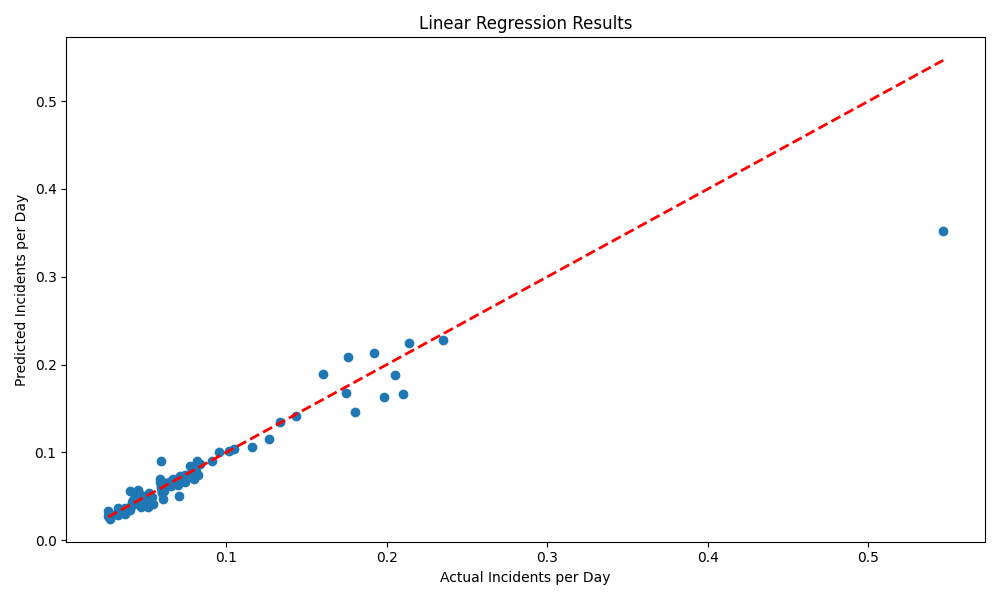
\includegraphics[width=.8\textwidth]{weekend_linear_regression_results.png}
    \caption{Valores reales y valores predichos por el modelo para los datos de fines de semana}
    \label{fig:weekend_reg_res}
\end{figure}

\begin{figure}[H]
    \centering
    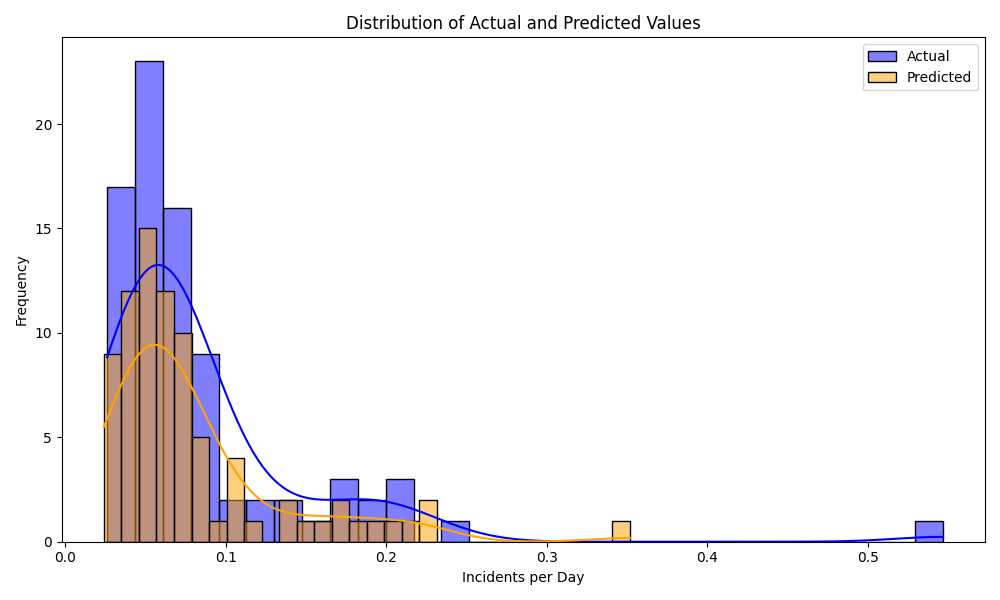
\includegraphics[width=.8\linewidth]{weekend_linear_regression_distribution.png}
    \caption{Distribución de valores reales y valores predichos por el modelo para los datos de fines de semana}
    \label{fig:weekend_reg_dist}
\end{figure}

Tras este análisis, podemos concluir que es un buen modelo de predicción y que prodría usarse con seguridad.

Por último, para poder aceptar o rechazar nuestra hipótesis, hemos comparado los incidentes en fines de semana o fuera de ellos mediante \textit{boxplots}, que pueden verse en la figura \ref{fig:weekend_boxplot}. Se puede observar con claridad que ambas distribuciones son prácticamente idénticas, lo que nos puede indicar que esta variable no es lo suficientemente significativa, y sí que lo son el estado y el año.

\begin{figure}[H]
    \centering
    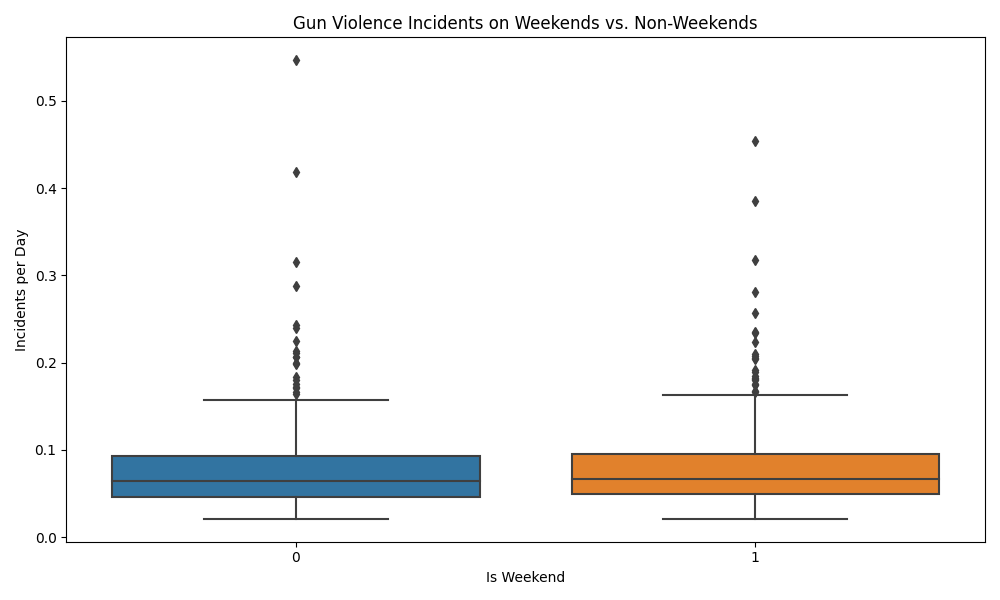
\includegraphics[width=.8\linewidth]{weekend_boxplot.png}
    \caption{\textit{Boxplots} del número de incidentes por día y 100.000 habitantes según si ocurren en fin de semana o no}
    \label{fig:weekend_boxplot}
\end{figure}

Además, hemos realizado un análisis estadístico mediante el método de mínimos cuadrados ordinarios sobre nuestro modelo de regresión lineal, para comprobar si la variable \textit{is\_weekend} es lo suficientemente significativa en el modelo. Este análisis nos ha resultado en un p-valor para \textit{is\_weekend} de 0,048. Tomando una confianza del 95\%, el p-valor es menor del 5\%, por lo que podemos rechazar la hipótesis de que el coeficiente poblacional es 0 e inclinarnos por la alternativa de que si ocurre o no en fin de semana es significativo para el modelo. Sin embargo, el valor es muy cercano al límite (0,05), y con la comparativa vista en la figura \ref{fig:weekend_boxplot} creemos que no podemos afirmar que existe una relación significativa entre el número de incidentes con armas y si es fin de semana o no.

\subsection{\textit{Clustering} con datos climáticos}

Para agrupar los incidentes según datos climáticos, nuestro algoritmo toma como entrada la temperatura y las precipitaciones medias en un mes, de manera que podemos clasificar los datos de cualquier región y en cualquier momento de manera más general (ya no utilizamos ni el estado ni el año).

Hemos dividido los datos en 3 grupos, que pueden observarse en la figura \ref{fig:clim_clusters}. Además, hemos incluido los valores medios para el número de incidentes por 100.000 habitantes, la temperatura media mensual y las precipitaciones medias mensuales para cada \textit{cluster} en la tabla \ref{tab:clim_clusters_medias}.

\begin{figure}[H]
    \centering
    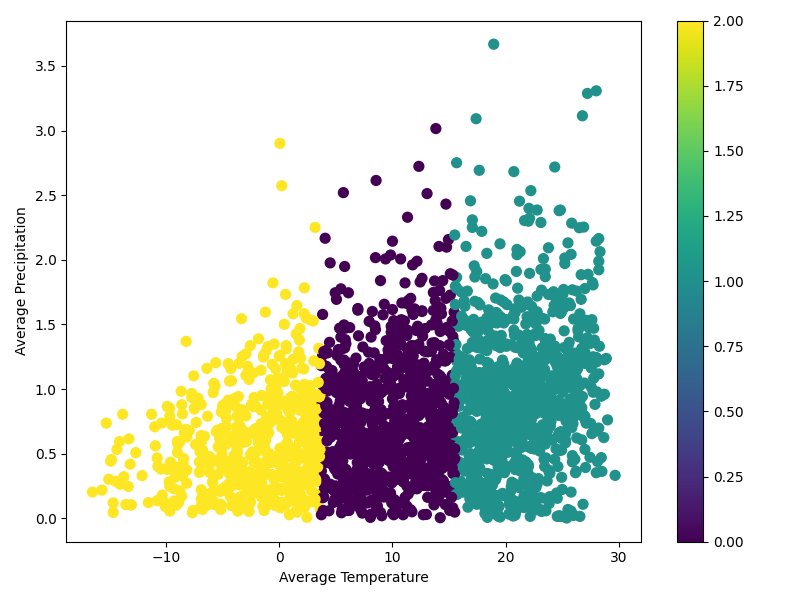
\includegraphics[width=.8\linewidth]{climate_clusters.png}
    \caption{Agrupación de los datos en \textit{clusters} según temperatura y precipitaciones}
    \label{fig:clim_clusters}
\end{figure}

\begin{table}[H]
    \centering
\begin{tabular}{|c|c|c|c|}
\hline
\textbf{cluster} & \textbf{n\_incidents} & \textbf{average\_temperature} & \textbf{average\_precipitation} \\ \hline
2                & 1.301505              & -2.401835                     & 0.596606                        \\ \hline
0                & 1.519505              & 9.773176                      & 0.795774                        \\ \hline
1                & 1.722896              & 21.194531                     & 0.938084                        \\ \hline
\end{tabular}
    \caption{Valores medios de las variables para cada \textit{cluster} según el clima}
    \label{tab:clim_clusters_medias}
\end{table}

Gracias a esta visualización y valores, podemos darle el siguiente significado a cada \textit{cluster}:

\begin{itemize}
    \item \textbf{Cluster 0}: temperatura baja-media y precipitaciones medias
    \item \textbf{Cluster 1}: temperatura media-alta y precipitaciones medias-altas
    \item \textbf{Cluster 2}: temperatura muy baja-baja y precipitaciones bajas
\end{itemize}

Podemos ver claramente que los \textit{clusters} con mayor temperatura tienen un mayor número de incidentes. Además, los \textit{clusters} con más precipitaciones tienen también un mayor número de incidentes. Sin embargo, la temperatura varía mucho más de un \textit{cluster} a otro, lo que puede ser debido a ser más significativa para la diferenciación en \textit{clusters}. Por tanto, podemos confirmar nuestra hipótesis de que existe una relación entre el número de incidentes con armas y la temperatura.

\subsection{Regresión con datos de pobreza}

El modelo de regresión lineal entrenado toma como características el estado, el año y la tasa de pobreza, y predice el número de incidentes por 100.000 habitantes para ese estado y año. Como se puede observar en los resultados de las métricas obtenidas al probar el modelo en la tabla \ref{tab:met_reg_pob}, los errores son bastante mayores que en el modelo de regresión para la primera hipótesis. Esto se debe, en parte, a que nuestra variable objetivo ya no se encuentra escalada por día (sólo por 100.000 habitantes), por lo que los valores de error deben ser mayores. Sin embargo, valores porcentuales como el MAPE y el $R^2$ nos indican el rendimiento relativo del modelo. Este modelo sólo explica un 63,28\% de la varianza de la variable objetivo, y tiene un MAPE del 20,14\%. Por tanto, este modelo tiene un rendimiento peor que el que usaba los fines de semana. En general, no es un modelo muy bueno, aunque podría ser aceptable para predicciones en contextos que no sean críticos y que permitan errores sin consecuencias graves.

\begin{table}[H]
    \centering
    \begin{tabular}{|c|c|}
        \hline
        \textbf{Métrica} & \textbf{Resultado} \\
        \hline
        Mean Squared Error & $255,33$ \\
        \hline
        Root Mean Squared Error & $15,98$ \\
        \hline
        Mean Absolute Error & $5,561$ \\
        \hline
        Mean Absolute Percentage Error & $20,14\%$ \\
        \hline
        $R^2$ & $63,28\%$ \\
        \hline
    \end{tabular}
    \caption{Métricas de rendimiento del modelo de regresión lineal con tasa de pobreza}
    \label{tab:met_reg_pob}
\end{table}

La figura \ref{fig:pob_reg_res} muestra los valores reales y los predichos por el modelo de una manera más clara. Podemos comprobar que, de nuevo, la precisión del modelo es mayor cuando el número de incidentes es menor, y el error va aumentándose con el número de incidentes. Además, la figura \ref{fig:pob_reg_dist} muestra la distribución de valores reales y predichos. Aquí, podemos observar de nuevo que el modelo siempre predice valores menores que los reales.

\begin{figure}[H]
    \centering
    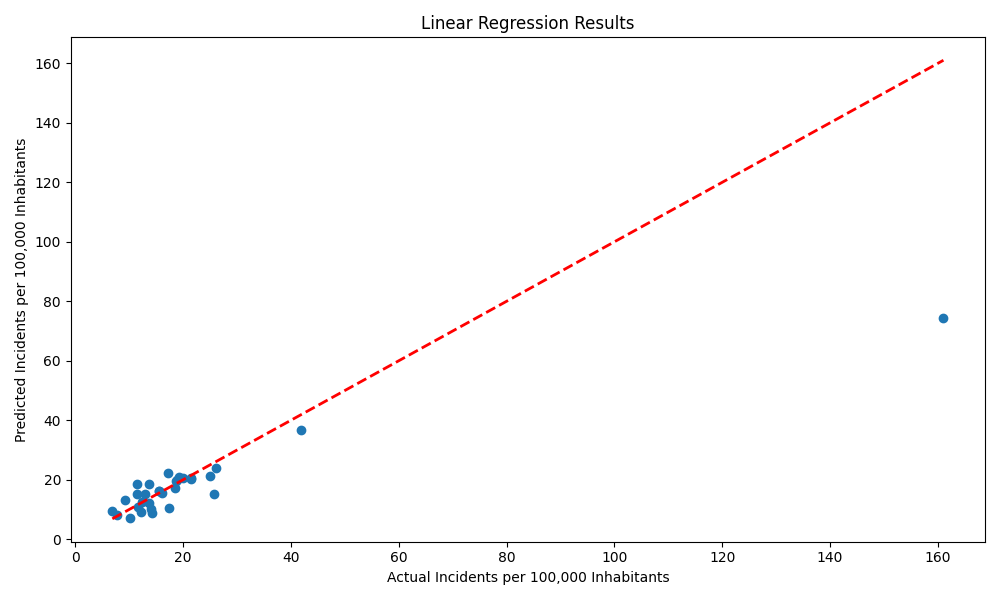
\includegraphics[width=.8\textwidth]{poverty_linear_regression_results.png}
    \caption{Valores reales y valores predichos por el modelo para los datos de pobreza}
    \label{fig:pob_reg_res}
\end{figure}

\begin{figure}[H]
    \centering
    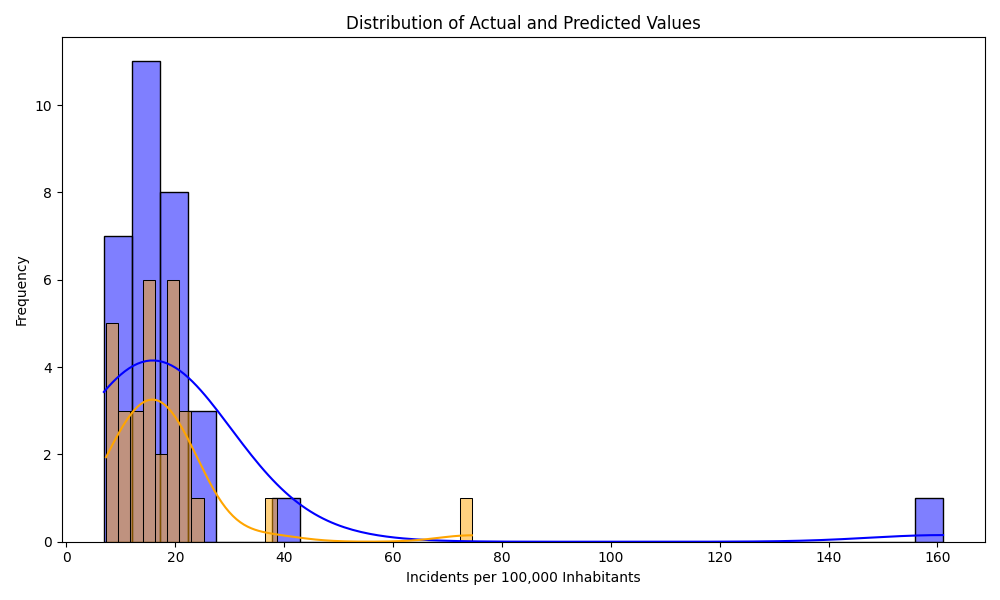
\includegraphics[width=.8\linewidth]{poverty_linear_regression_distribution.png}
    \caption{Distribución de valores reales y valores predichos por el modelo para los datos de pobreza}
    \label{fig:pob_reg_dist}
\end{figure}

Tras este análisis, podemos concluir que no es un gran modelo de predicción, y que podría usarse dependiendo del contexto, i.e. si no se necesitan predicciones exactas.

Por último, para poder aceptar o rechazar nuestra hipótesis, hemos realizado otro análisis estadístico mediante el método de mínimos cuadrados ordinarios sobre nuestro modelo de regresión lineal, para comprobar si la variable \textit{poverty\_rate} es lo suficientemente significativa en el modelo. Este análisis nos ha resultado en un p-valor para \textit{poverty\_rate} de 0,857. Tomando una confianza del 95\%, el p-valor es mayor del 5\% (además de ser extremadamente alto, siendo casi 1), por lo que podemos aceptar la hipótesis de que el coeficiente poblacional es 0 e inclinarnos por la alternativa de la tasa de pobreza no es significativo para el modelo. Esto nos indica que nuestro modelo da una mayor importancia para sus predicciones al estado y el año, siendo la tasa de pobreza poco relevante.

Por tanto, de momento no podemos afirmar que existe una relación significativa entre el número de incidentes con armas y la tasa de pobreza. Aprovecharemos el análisis final con datos combinados para reafirmarnos en esta idea o para rechazarla.

\subsection{\textit{Clustering} con datos de leyes}

Para agrupar los incidentes según datos de leyes, nuestro algoritmo toma como entrada el total de leyes vigentes y el total de cada una de las categorías de leyes. De esta manera, al no incluir el estado y el año podemos clasificar los datos independientemente de estos.

Por la gran cantidad de variables, hemos utilizado PCA para reducirlas a 3 componentes. Hemos dividido los datos en 3 grupos, que pueden observarse en la figura \ref{fig:ley_clusters}. Al haber reducido las características, este gráfico no nos proporciona una buena visualización de los grupos dependiendo de las variables que en realidad tenemos. Para analizar mejor los grupos, hemos incluido de nuevo los valores medios para el número de incidentes por 100.000 habitantes y cada una de las variables de leyes para cada \textit{cluster} en la tabla \ref{tab:ley_clusters_medias}.

\begin{figure}[H]
    \centering
    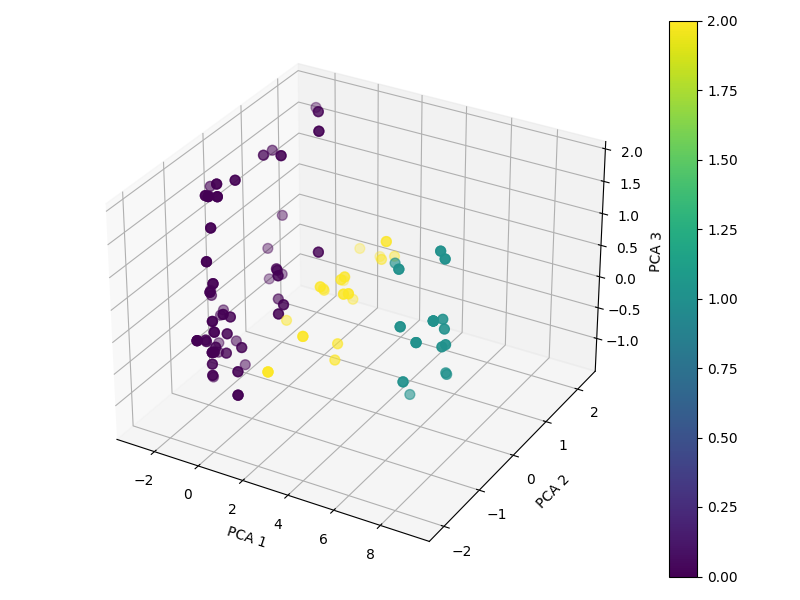
\includegraphics[width=.8\linewidth]{laws_clusters.png}
    \caption{Agrupación de los datos en \textit{clusters} según leyes de regulación de armas}
    \label{fig:ley_clusters}
\end{figure}

\begin{table}[H]
    \centering
\adjustbox{max width=\textwidth}{
\begin{tabular}{|c|c|c|c|c|c|c|c|c|c|c|c|c|c|c|c|c|}
\hline
\textbf{cluster} & \textbf{n\_incidents} & \textbf{lawtotal} & \textbf{laws\_1} & \textbf{laws\_2} & \textbf{laws\_3} & \textbf{laws\_4} & \textbf{laws\_5} & \textbf{laws\_6} & \textbf{laws\_7} & \textbf{laws\_8} & \textbf{laws\_9} & \textbf{laws\_10} & \textbf{laws\_11} & \textbf{laws\_12} & \textbf{laws\_13} & \textbf{laws\_14} \\ \hline
1                & 16.35 & 79.97 & 9.12 & 9.50 & 7.38 & 7.75 & 3.25 & 5.84 & 5.50 & 4.53 & 6.00 & 2.53 & 1 & 2.25 & 1 & 14.31 \\ \hline
2                & 17.54 & 33.35 & 4.20 & 2.83 & 3.57 & 5.75 & 0.50 & 2.10 & 4.60 & 0.10 & 1.90 & 0.75 & 0.88 & 0.20 & 0.60 & 5.38 \\ \hline
0                & 19.05 & 11.36 & 0.62 & 0.56 & 2 & 0.27 & 0.12 & 1.83 & 2.95 & 0 & 0.47 & 0.34 & 0.30 & 0 & 0.09 & 1.80 \\ \hline
\end{tabular}
}
    \caption{Valores medios de las variables para cada \textit{cluster} según leyes de regulación de armas (puede verse con un mejor tamaño en los \textit{notebooks})}
    \label{tab:ley_clusters_medias}
\end{table}

Gracias a estos valores, podemos darle el siguiente significado a cada \textit{cluster}:

\begin{itemize}
    \item \textbf{Cluster 0}: cantidad de leyes vigentes baja
    \item \textbf{Cluster 1}: cantidad de leyes vigentes muy alta
    \item \textbf{Cluster 2}: cantidad de leyes vigentes media
\end{itemize}

Podemos ver claramente que los \textit{clusters} con más leyes de regulación de armas vigentes tienen un mayor número de incidentes. Además, gracias a la división en categorías de las leyes, podemos hacer un pequeño análisis de varianza para ver que leyes varían más entre \textit{clusters}, i.e. son más significativas. Para ello, la tabla \ref{tab:leyes_std} muestra las desviaciones estándar de cada variable entre \textit{clusters}, i.e. cuánto varían.

Obviando el número total de leyes, podemos ver que las más importantes son las categorías 14, 2 y 1, que corresponden a leyes de regulación según antecedentes de violencia doméstica, de regulación a compradores y de regulación a vendedores, respectivamente. Por otro lado, las menos importantes son las categorías 11, 13 y 10, que corresponden a leyes que permiten abrir fuego como defensa propia sin el deber de intentar retirarse antes, leyes que permiten la inmunidad de los vendedores respecto a los daños causados con las armas que han vendido, y leyes que regulan el tráfico de armas, respectivamente.

\begin{table}[H]
    \centering
\begin{tabular}{|c|c|}
\hline
\textbf{Variable} & \textbf{Desviación estándar} \\ \hline
lawtotal          & 35.033655                    \\ \hline
laws\_14          & 6.446223                     \\ \hline
laws\_2           & 4.646745                     \\ \hline
laws\_1           & 4.267830                     \\ \hline
laws\_4           & 3.875011                     \\ \hline
laws\_9           & 2.870923                     \\ \hline
laws\_3           & 2.763188                     \\ \hline
laws\_8           & 2.587734                     \\ \hline
laws\_6           & 2.244060                     \\ \hline
laws\_5           & 1.706300                     \\ \hline
laws\_7           & 1.291560                     \\ \hline
laws\_12          & 1.245325                     \\ \hline
laws\_10          & 1.163547                     \\ \hline
laws\_13          & 0.454162                     \\ \hline
laws\_11          & 0.375108                     \\ \hline
\end{tabular}
    \caption{Desviaciones estándar de las variables de leyes entre \textit{clusters}.}
    \label{tab:leyes_std}
\end{table}

\subsection{\textit{Clustering} para análisis combinado}

Para agrupar los incidentes según datos climáticos, de pobreza y de leyes, nuestro algoritmo toma como entrada todos estos datos sin estado ni año. Por tanto, toma como entrada la temperatura media anual, las precipitaciones medias anuales, la tasa de pobreza, el total de leyes vigentes y el total de cada una de las categorías de leyes. De esta manera, al no incluir el estado y el año podemos clasificar los datos independientemente de estos.

Por la gran cantidad de variables, hemos utilizado PCA para reducirlas a 3 componentes. Hemos dividido los datos en 3 grupos, que pueden observarse en la figura \ref{fig:comb_clusters}. Al haber reducido las características, este gráfico no nos proporciona una buena visualización de los grupos dependiendo de las variables que en realidad tenemos. Para analizar mejor los grupos, hemos incluido de nuevo los valores medios para el número de incidentes por 100.000 habitantes y cada una de las variables cada \textit{cluster} en la tabla \ref{tab:comb_clusters_medias}.

\begin{figure}[H]
    \centering
    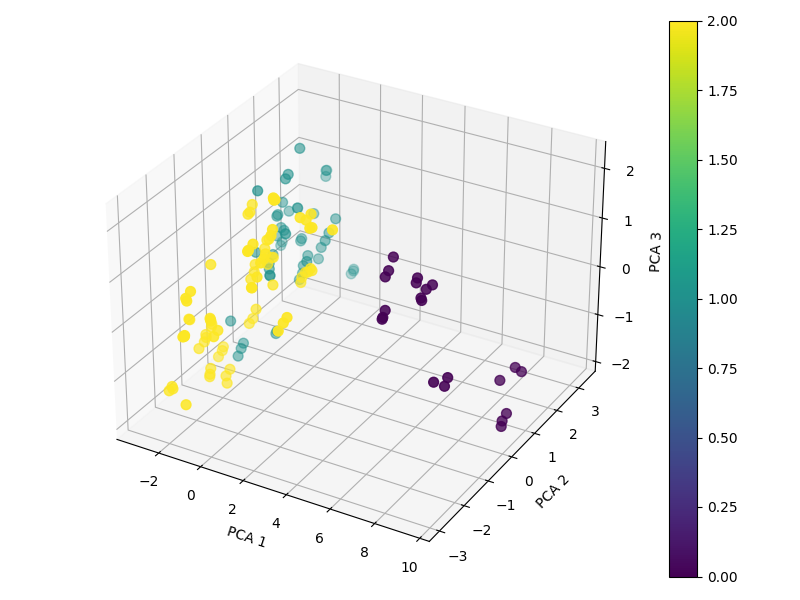
\includegraphics[width=.8\linewidth]{combined_clusters.png}
    \caption{Agrupación de los datos en \textit{clusters} según combinación de factores anteriores}
    \label{fig:comb_clusters}
\end{figure}

\begin{table}[H]
    \centering
\adjustbox{max width=\textwidth}{
\begin{tabular}{|c|c|c|c|c|c|c|c|c|c|c|c|c|c|c|c|c|c|c|c|}
\hline
\textbf{cluster} & \textbf{n\_incidents} & \textbf{average\_temperature} & \textbf{average\_precipitation} & \textbf{poverty\_rate} & \textbf{lawtotal} & \textbf{laws\_1} & \textbf{laws\_2} & \textbf{laws\_3} & \textbf{laws\_4} & \textbf{laws\_5} & \textbf{laws\_6} & \textbf{laws\_7} & \textbf{laws\_8} & \textbf{laws\_9} & \textbf{laws\_10} & \textbf{laws\_11} & \textbf{laws\_12} & \textbf{laws\_13} & \textbf{laws\_14} \\ \hline
2                & 17.64 & 8.94 & 0.67 & 0.13 & 18.95 & 2.04 & 1.42 & 2.65 & 2.45 & 0.23 & 1.59 & 3.14 & 0.04 & 0.88 & 0.62 & 0.64 & 0.08 & 0.35 & 2.82 \\ \hline
0                & 18.96 & 11.76 & 0.83 & 0.12 & 80.57 & 9.29 & 8.76 & 7 & 8 & 3.57 & 6.05 & 5.43 & 5.19 & 6.14 & 2.86 & 1 & 2.14 & 1 & 14.14 \\ \hline
1                & 21.75 & 16.86 & 1.03 & 0.18 & 12.94 & 0.56 & 0.56 & 2 & 0.25 & 0.19 & 2.35 & 3.44 & 0 & 0.69 & 0.19 & 0.08 & 0 & 0 & 2.63 \\ \hline
\end{tabular}
}
    \caption{Valores medios de las variables para cada \textit{cluster} según combinación de factores anteriores (puede verse con un mejor tamaño en los \textit{notebooks})}
    \label{tab:comb_clusters_medias}
\end{table}

Gracias a estos valores, podemos darle el siguiente significado a cada \textit{cluster}:

\begin{itemize}
    \item \textbf{Cluster 0}: incidentes medios
    \begin{itemize}
        \item Temperatura baja-media
        \item Precipitaciones medias
        \item Tasa de pobreza baja
        \item Cantidad de leyes vigentes muy alta
    \end{itemize}
    \item \textbf{Cluster 1}: incidentes más altos
    \begin{itemize}
        \item Temperatura media
        \item Precipitaciones altas
        \item Tasa de pobreza alta
        \item Cantidad de leyes vigentes baja-media
    \end{itemize}
    \item \textbf{Cluster 2}: incidentes más bajos
    \begin{itemize}
        \item Temperatura baja
        \item Precipitaciones medias
        \item Tasa de pobreza baja
        \item Cantidad de leyes vigentes baja
    \end{itemize}
\end{itemize}

Gracias a este análisis combinado, podemos ver que el número de incidentes aumenta con la temperatura y la tasa de pobreza, y se reduce con las leyes de regulación de armas. Sin embargo, ahora vemos que la tasa de pobreza si que es alta cuando los incidentes son altos, pero se mantiene igual con incidentes más bajos o medios. Lo mismo ocurre con el número de leyes: el número de leyes es alto cuando los incidentes son altos, pero se mantiene igual con incidentes más bajos o medios. Por tanto, podemos concluir:

\begin{enumerate}
    \item El número de incidentes de violencia con armas aumenta con la temperatura.
    \item El número de incidentes de violencia con armas aumenta con tasas de pobreza muy altas, pero no depende de estas cuando son bajas.
    \item El número de incidentes de violencia con armas se reduce con muchas leyes de regulación vigentes, pero no depende de estas cuando no hay muchas.
\end{enumerate}

\end{document}